% !TeX root=main.tex

\chapter{مقدمه}
\pagenumbering{arabic}



در این بخش سعی می‌شود مفاهیم و تعاریف اولیه‌ی مورد نیاز برای ورود به مسئله‌ی اصلی به‌صورت مختصر تبیین گردد، سپس به تعریف مسئله می‌پردازیم.

\section{دارو}
در دانش پزشکی به هر ماده‌ای که برای درمان، تسکین علائم، تشخیص بیماری یا پیش‌گیری از آن به‌کار رود و بر ساختار یا کارکرد ارگانیسم زنده اثر گذارد و پس از ورود به بدن عملکرد بدن را تصحیح کند، دارو 
\LTRfootnote{Drug}
گفته می‌شود. در تعریفی دیگر دارو به ماده‌ای گفته می‌شود که با اثر بر گیرنده‌ای خاص در داخل، خارج یا دیواره‌ی سلول باعث شروع یا مهار عملکردی خاص ‌گردد و قدرت اثر دارو با میزان و تعداد این برهم‌کنش نسبت مستقیم دارد. البته داروهایی که  اثر موضعی دارند مانند آنتی اسیدها و ضدعفونی کننده‌های موضعی و مواد حاجب در این تعریف نمی‌گنجند 
\cite{Basic2018}.
امروزه اطلاعات دارو‌ها به طور گسترده در پایگاه‌داده‌های دارو قابل دسترسی می‌باشد که به تعدادی از مهم‌ترین آن‌ها در بخش
\ref{data base} 
اشاره می‌کنیم.
 
\section{داروشناسی}
داروشناسی
\LTRfootnote{Pharmacology} 
دانش بررسی واکنش مواد شیمیایی در سیستم‌های زیستی است. داروشناسی پزشکی
\LTRfootnote{Medical Pharmacology}
بخشی از داروشناسی که در ارتباط با استفاده از مواد شیمیایی در پیشگیری، تشخیص و درمان بیماری، به ویژه در انسان است. دو حوزه اصلی داروشناسی، فارماکودینامیک 
\LTRfootnote{Pharmacodynamic}
و فارماکوکینتیک
\LTRfootnote{Pharmacokinetic} 
هستند. به‌طور خلاصه فارماکودینامیک مطالعه‌ی اثرات داروها بر بدن و فارماکوکینتیک، اثر و رفتار بدن برروی داروهاست. به‌عبارت دیگر فارماکودینامیک به مبحث واکنش‌های دارو در مواجهه با گیرنده‌های زیستی و فارماکوکینتیک به بحث و تعریف جذب، توزیع، متابولیسم و دفع دارو در سیستم‌های زیستی می‌پردازد
\cite{katzung2019katzung}.
داروشناسی و داروسازی
\LTRfootnote{Pharmacy} 
دو واژه جدا از هم هستند که گاهی به ‌اشتباه به‌جای هم به‌کار می‌روند. داروشناسی نوع رفتار دارو و سیستم‌ زیستی (بدن) است ولی داروسازی در رابطه با مواد اولیه، آماده‌سازی، توزیع و مقدار
\LTRfootnote{Dose}
مصرف داروهای بی‌خطر و موثر است.
\subsection{برهم‌کنش فارماکوکینتیک}

فارماکوکینتیک تأثیر سیستم‌های زیستی بر داروها را نشان می‌دهد. عمده‌ی فرآیندهای دخیل در فارماکوکینتیک جذب، توزیع، متابولیسم و دفع هستند. بیماری‌های مختلف می‌توانند پارامترهای استاندارد فارماکوکینتیک معمول را تغییر دهند. در صورت مشخص شدن پارامترهای فارماکوکینتیک بیمار، تنظیم مقدار مصرف دارو برای یک بیمار خاص قابل محاسبه است
\cite{katzung2019katzung}.
وقتی دو دارو با‌هم مصرف می‌شوند، روند جذب، توزیع، متابولیسم یا دفع یکی یا هر‌دوی آن‌ها ممکن‌ است با رفتار مورد انتظار آن‌ها در حالتی که دارو به تنهایی مصرف می‌شود، متفاوت باشد. چنین تفاوت‌هایی را ناشی از برهم‌کنش‌های فارماکوکینتیک می‌دانیم که عبارتند‌ از:
\par
\subsubsection*{برهم‌کنش بر اساس جذب: }
این امکان وجود دارد که فرآیند جذب
\LTRfootnote{Absorption}
دارو (از دیواره‌ی روده) درصورتی‌که با داروی دیگری ترکیب شود، کاهش یا افزایش یابد. در فرآیند جذب از دیواره‌ی روده، برخی از داروهای تنگ‌کننده ‌عروق، به محض استفاده (ورود به بدن) با عملکرد موقتی در موضع و با محدودکردن اندازه ‌رگ‌ها باعث کند شدن جذب دیگر داروها می‌شوند. گاهی پزشکان از این پدیده بهره‌ می‌گیرند، برای مثال برخی بی‌حس‌کننده‌های موضعی را با داروهای آلفا۱-آدرنرژیک (اپی‌نفرین، نوراپی‌نفرین، سینفرین) که تنگ‌کننده عروق هستند، برای کندکردن جذب و تداوم اثر دارو در موضع مورد نیاز، به‌کار می‌برند
\citep{Rescigno2003}.

\par
\subsubsection*{برهم‌کنش بر‌اساس توزیع: }
توزیع
\LTRfootnote{Distribution}
دارو ممکن است تحت تاثیر داروهایی که دارای اثر رقابتی بر جایگاه اتصال پروتین‌های پلاسما می‌باشند قرار گیرد. به‌طور مثال داروهای آنتی‌باکتریال سولفوناميدی قابليت جابجايی داروهايی نظير متوتروکسات، فنی‌توئين، سولفونيل اوره‌ها و وارفارين از آلبومين پلاسما را دارند. یک دارو با ایجاد تغییراتی در محیط فیزیکی و در محیط  توزیع داروی دیگر، باعث تغییر انتشار داروی دوم می‌شود. برای مثال ديورتيک‌ها می‌توانند از طريق کاهش آب کلی بدن، ميزان انتشار آمينوگليکوزيدها را کاهش دهند و باعث تشديد سميت دارويی آمينوگليکوزيدها و ليتيوم بدليل افزايش غلظت پلاسمايی آنان شوند.

\par
\subsubsection*{برهم‌کنش بر اساس متابولیسم:‌ }
این نوع برهم‌کنش‌ها به‌خوبی اثبات‌ شده‌اند و از اهمیت بالای بالینی برخوردارند. متابولیسم
\LTRfootnote{Metabolism}
اکثر دارو‌ها در کبد توسط آنزیم سیتوکروم
\lr{P450}
صورت می‌گیرد. متابولیسم یک دارو در صورت تجویز همزمان با داروهایی که اثر القاکنندگی بر این آنزیم‌ها دارند، افزایش می‌یابد و  متابولیسم یک دارو در صورت تجویز همزمان با داروهایی که اثر مهارکنندگی بر این آنزیم‌ها دارند، کاهش می‌یابد. 

\par
\subsubsection*{برهم‌کنش بر‌اساس دفع: }
دفع
\LTRfootnote{Elimination}
بسیاری از داروها از طریق ادرار و سیستم کلیوی صورت می‌گیرد. برای مثال دفع یک دارو در صورت استفاده همزمان با داروهای کاهنده جريان خون کليوی، کاهش می‌یابد و یا مصرف هم‌زمان یک دارو با داروهای تغيير‌دهنده‌ی
\lr{PH}
ادرار، ميزان يونيزاسيون آن دارو را کاهش‌ می‌دهد.


\subsection{برهم‌کنش فارماکوداینامیک}
ممکن‌ است استفاده هم‌زمان دو دارو منجر به افزایش تاثیرات هر یک از آن‌ها شود یا برعکس ممکن‌ است اثرات یکدیگر را سرکوب کنند. به‌چنین تاثیرات افزایشی یا کاهشی داروها بر روی یکدیگر، برهم‌کنش‌های فارماکوداینامیک می‌گوییم که عبارتند از:

\subsubsection*{برهم‌کنش بر‌اساس اثر آنتاگونیسم: }

ساده‌ترین نوع برهم‌کنش دارویی است که اغلب قابل پیش‌بینی است. گاهی اوقات جذب یک دارو مانع جذب بعضی داروهای دیگر می‌گردد، این پدیده را آنتاگونیسم یا رقابت‌کنندگی\LTRfootnote{Antagonism}گویند\cite{kenakin1997pharmacologic}.
برای مثال دارو‌های ضد التهابی غیراستروئیدی
\lr{NSAIDs}
اثر ضد فشار داروی مهارکننده‌ی
\lr{ACEIs}
را از طریق کاهش دفع سديم، کم می‌کنند.

\subsubsection*{برهم‌کنش بر‌اساس اثر سینرژیسم: }
گاهی جذب یک دارو باعث تشدید و افزایش شدت جذب داروی دیگر می گردد، به این پدیده سینرژیسم یا تشدیدکنندگی\LTRfootnote{Synergnism}گویند\cite{chou2006theoretical}.
جمع‌جبری اثرات دو دارو، ممکن‌ است بر يک گيرنده‌ی خاص عمل نمايند. اگر مجموع اثرات دو دارو با هم از جمع اثر هر دارو  به‌تنهايی بيشتر باشد تداخل فوق سینرژیسم یا تشدید‌کنندگی می‌باشد.                

\section{پایگاه داده‌های دارو
\label{data base}}
 
اطلاعات دارویی مورد نیاز برای حل مسائل مختلف مرتبط با دارو، در پایگاه داده‌های معروفی به شرح زیر موجود هستند. 
 
\begin{figure}[h!]
	\centering
	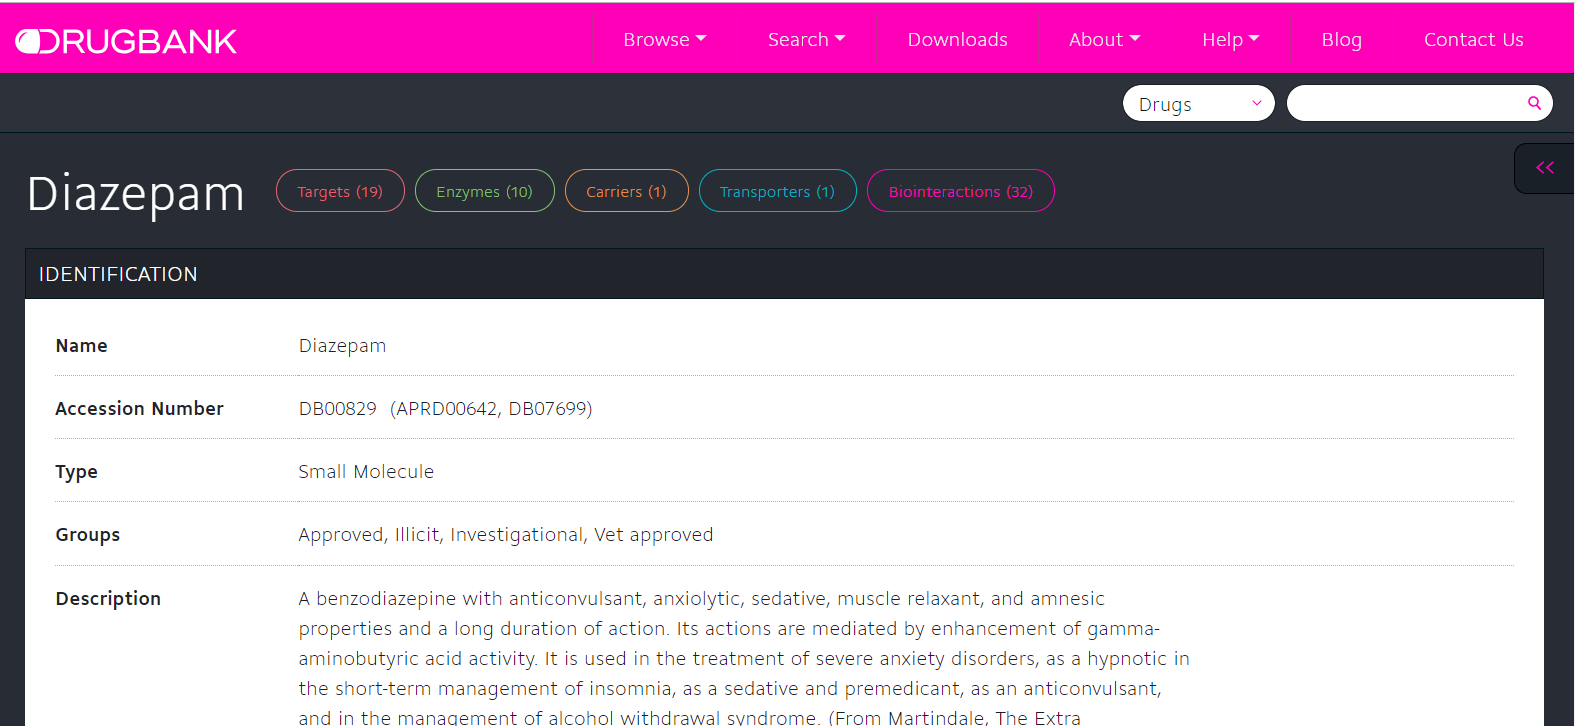
\includegraphics[scale=0.48]{section1/di.jpg}
	\caption{
قسمتی از نمایش اطلاعات داروی دیازپام در پایگاه داده‌ی
DrugBank}
	\label{fs1}
\end{figure}


\subsection{DrugBank}

\lr{DrugBank}
\cite{law2013drugbank,wishart2007drugbank,knox2010drugbank,wishart2006drugbank}:
یکی از منابع مهم تحقیقاتی بیوانفورماتیک می‌باشد که در آن اطلاعات دارو-هدف
\LTRfootnote{Drug-Target}،
آنزیم‌های دارو، انتقال‌ دهنده‌های دارو
‌\LTRfootnote{Drug Transporters}،
عوارض جانبی
\LTRfootnote{Side Effect}
دارو، برهم‌کنش‌های شناخته شده‌ی دارو با دیگر داروها و... موجود می‌باشد. درشکل
\ref{fs1} 
قسمتی از  اطلاعات داروی دیازپام
\LTRfootnote{Diazepam} 
نشان‌ داده‌ شده‌ است و در شکل 
\ref{fs2} 
قسمتی از اطلاعات برهم‌کنش داروی دیازپام با دیگر داروها نمایش داده شده‌ است. 

\begin{figure}[h!]
	\centering
	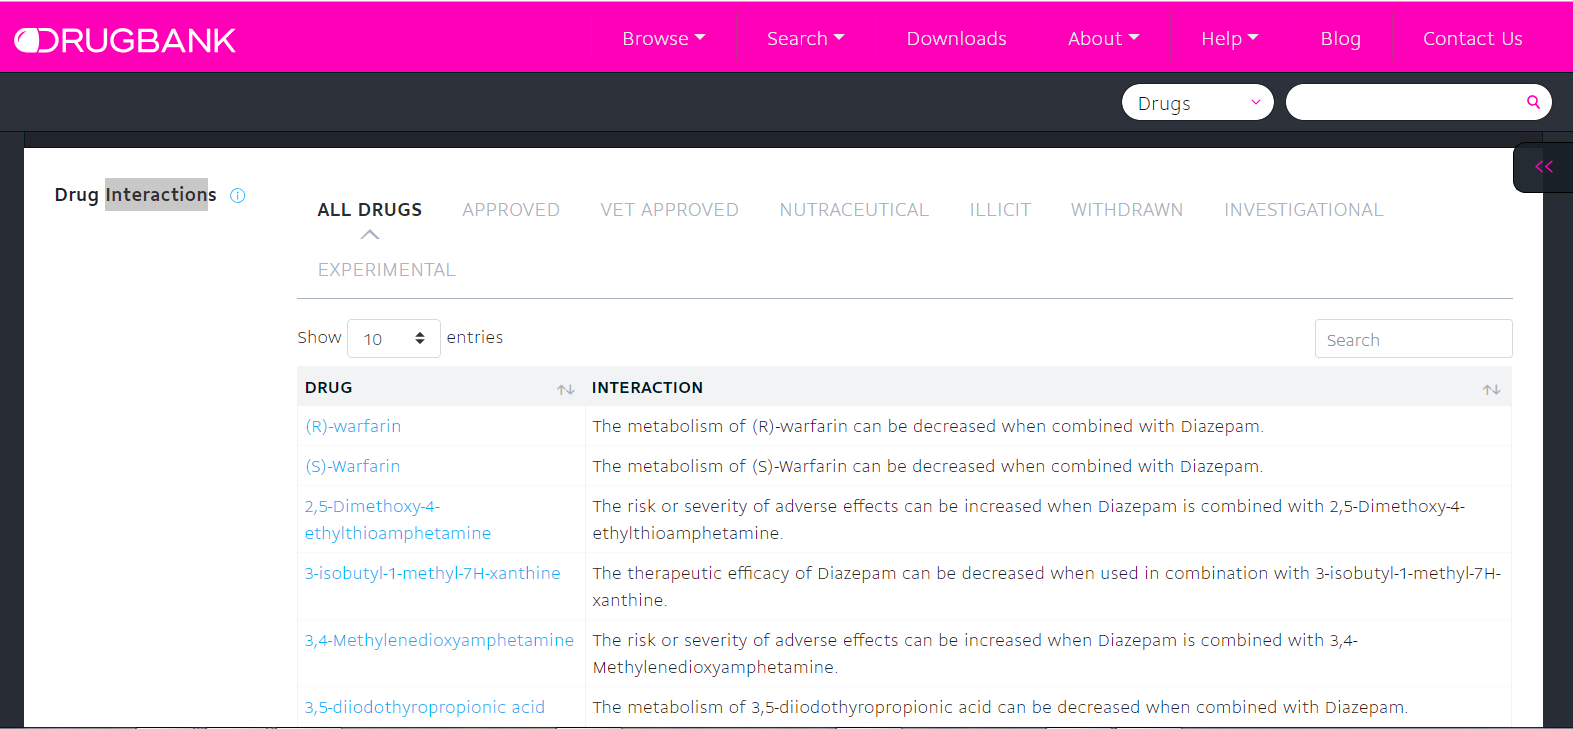
\includegraphics[scale=0.48]{section1/ddidi.png}
	\caption{
نمایش قسمتی از اطلاعات برهم‌کنش داروی دیازپام با دیگر داروها
	}
	\label{fs2}
\end{figure}

\subsection{KEGG}

\lr{KEGG}\LTRfootnote{Kyoto Encyclopedia of Genes \& Genomes}\cite{ogata1999kegg, kanehisa2000kegg}:
پایگاه داده‌ای مربوط به اطلاعات زیستی‌است که اولین بار توسط مینورور کانهیزا
\LTRfootnote{Minoru Kanehisa}
پروفسور موسسه‌ی تحقیقات شیمی در دانشگاه کیوتو در سال ۱۹۹۵ هم‌زمان با پروژه ژنوم درست شد. به منظور استفاده از تحلیل کامپیوتری برای تفسیر نتایج حاصل از پروژه ژنوم مینورور شروع به ساخت
\lr{KEGG Pathway}
کرد. در این پایگاه داده توسط دانش به‌دست آمده از آزمایش‌های مختلف، نقشه و مسیرهای متابولیکی ترسیم شده‌‌است و همچنین تعدادی از عملکرد‌های سلول‌ها و ارگانیزم‌ها به‌صورت جزئی به تصویر کشیده‌ شده‌‌است. هر نقشه شامل یکسری واکنش بین بیومولکول‌های مختلف می‌باشد که طوری طراحی شده‌است که از آن می‌شود اطلاعاتی در مورد ژن‌ها و پروتئین‌های دخیل در آن یافت. در این پایگاه‌داده می‌توان مسیرهای مختلف را با هم مقایسه و تحلیل کرد و به‌طور کلی از آن‌ها اطلاعات سودمندی استخراج کرد.
بر طبق نظر سازنده‌، 
\lr{KEGG} 
به صورت یک کامپیوتر ارائه دهنده‌ی سیستم‌های بیولوژیکی می‌باشد که دیاگرام‌ها و واحدهای متصل به هم ایجاد می‌کند. دیاگرام‌ها شامل ژن‌ها و عملکرد پروتئین‌های مرتبط، واکنش‌های بین مولکولی هستند. همچنین
\lr{KEGG} 
منبع مناسبی برای مسیرهای پروتئین 
\LTRfootnote{Protein Pathways}
 می‌باشد. در شکل 
\ref{fs3} 
صفحه‌ی اول این پایگاه داده که یک معرفی از آن می‌باشد نمایش داده شده است.

\begin{figure}[h!]
	\centering
	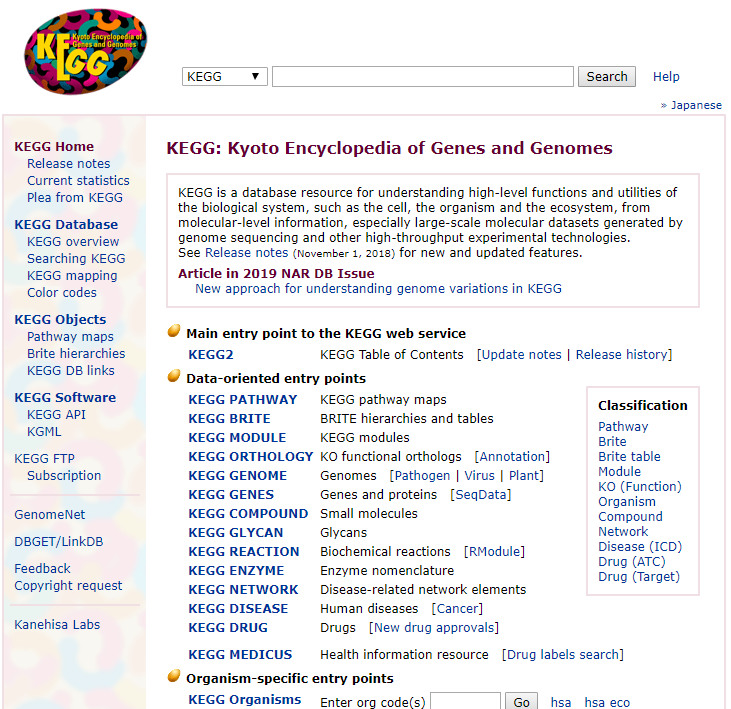
\includegraphics[scale=0.7]{section1/kegg1.PNG}
	\caption{ 
صفحه اول پایگاه داده KEGG}
	\label{fs3}
\end{figure}

\subsection{TWOSIDES}

\lr{TWOSIDES}\cite{Tatonetti2012}:
بانک اطلاعاتی عمومی حاوی عوارض‌جانبی ناشی از برهم‌کنش دارو–دارو  است. این بانک اطلاعاتی حاوی 868221 ارتباط بین 59220 جفت دارو و 1301 عوارض‌جانبی است. این ارتباطات فقط به مواردی محدود می شوند كه به‌طور واضح به‌هیچ یك از داروها اختصاص نیافته است (ارتباط‌های تحت پوشش
\lr{OFFSIDES}).
این پایگاه داده حاوی 3782910 ارتباط مهم دیگر است که، جفت داروها دارای نمره عوارض‌جانبی بالاتری هستند که با استفاده از نسبت گزارش متناسب 
\LTRfootnote{Proportional Reporting Ratio(PRR)}،
تعیین می‌شوند.

\subsection{FAERS}

\lr{FAERS}\LTRfootnote{FDA Adverse Event Reporting System} :
سیستم گزارش‌دهی رویدادهای ناخواسته‌ی سازمان غذا و دارو پایگاه داده‌ای، حاوی اطلاعات مربوط به عوارض‌جانبی ارسال شده به سازمان غذا و دارو\LTRfootnote{Food and Drug Adminstration(FDA)}است. این پایگاه داده، توسط
\lr{FDA}\LTRfootnote{http://www.fda.gov}،
به‌منظور پشتیبانی از برنامه‌ی نظارت بر ایمنی پس از بازاریابی برای داروها و محصولات بیولوژیکی درمانی طراحی شده است. داده‌های استخراج شده از 
\lr{FAERS}
 و 
\lr{TWOSIDES} 
مجموعه داده‌ای است که فقط شامل عوارض‌جانبی است که به دلیل ترکیب داروها ایجاد می شود 
\cite{Zhang2015}.

\subsection{SIDER}

\lr{{SIDER}}\cite{kuhn2015sider}:
در این پایگاه داده اطلاعات عوارض جانبی دارو‌ها و نشانگان دارو وجود‌ دارد. این پایگاه داده حاوی اطلاعاتی در مورد داروهای بازار و واکنش‌های دارویی نامطلوب آن‌ها است. با وجود این‌که
\lr{SIDER}
منبع مهمی از عوارض جانبی شناخته شده است، اما اطلاعات آن محدود است
\cite{Zhang2015}.
زیرا:

الف) آزمایشات بالینی بر روی جمعیت نسبتاً کمی از بیماران انجام می‌شود و فقط عوارض‌جانبی متداول با اطمینان بالا در لیست دارویی مشاهده می‌شوند.

ب) از طرفی عارضه‌ی‌جانبی مشاهده ‌شده در طول آزمایشات بالینی ممکن است اتفاقی باشد و در واقع توسط دارو ایجاد نشده باشد. 

لازم به ذکر است، عوارض‌جانبی‌ که از این پایگاه ‌داده استخراج شده ‌است 
\lr{Labele Side Effect}
نامیده می‌شود.

در شکل 
\ref{fs5} 
نمایی از صفحه‌ی اول پایگاه داده‌ی
\lr{SIDER}
مشاهده می‌شود که می‌توان براساس نام دارو یا عارضه‌جانبی در این پایگاه ‌داده جستجو نمود. 
\begin{figure}[h!]
	\centering
	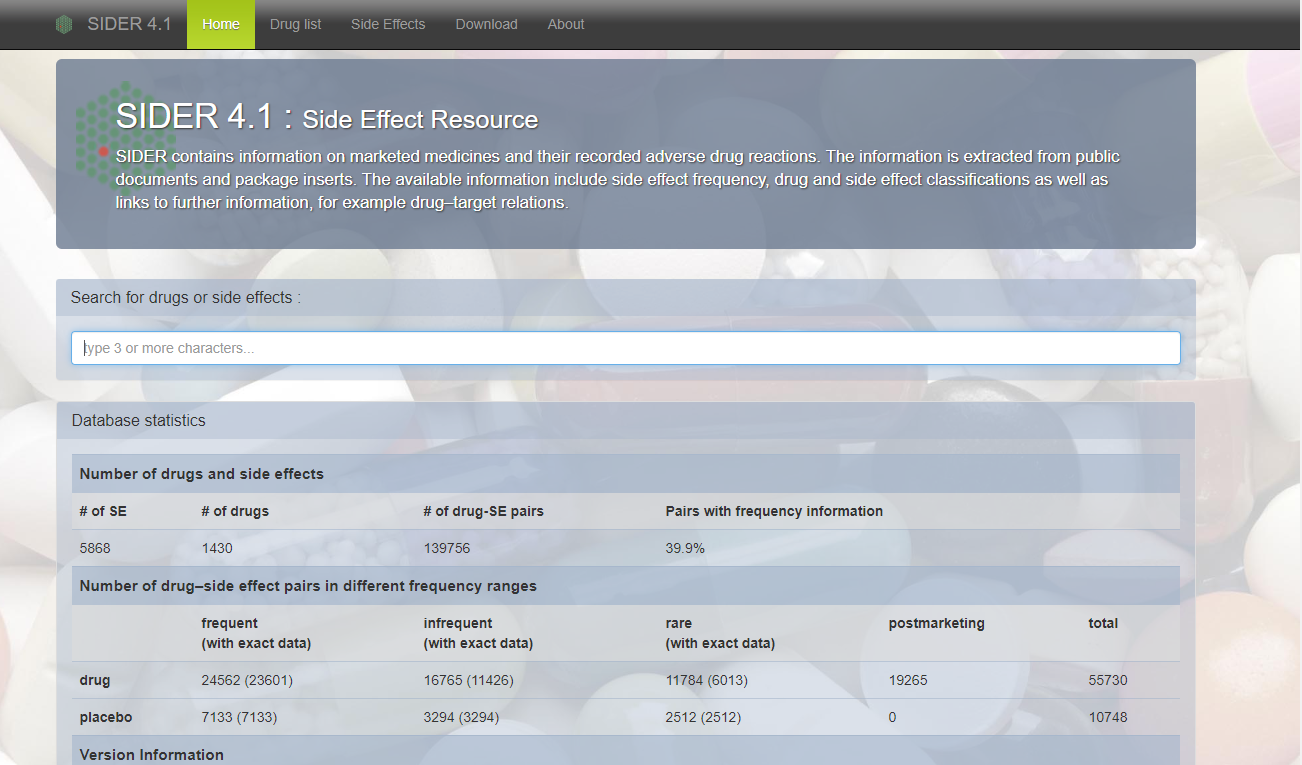
\includegraphics[scale=0.48]{section1/Sider1.png}
	\caption{ 
صفحه اول پایگاه داده SIDER}
	\label{fs5}
\end{figure}


\subsection{OFFSIDES}

مجموعه‌ای از عوارض‌جانبی داروها است که حاصل کاوش عوامل مخدوش کننده مانند مصرف داروهای همزمان، اطلاعات دموگرافیک بیمار و تاریخچه پزشکی بیمار از پایگاه‌داده‌ی 
\lr{FAERS} 
است. در این پایگاه‌داده 1332 دارو و 10093 عارضه‌جانبی وجود دارد. لازم به ذکر است، عوارض‌جانبی استخراج شده از 
\lr{OFFSIDES}
 با عنوان 
\lr{Off-Label Side Effect}
نامگذاری ‌می‌شود
\cite{Tatonetti2012}.

\subsection{PubChem}

پایگاه داده مربوط به مولکول‌های شیمیایی است که توسط موسسه ملی سلامت در ایالات متحده
\LTRfootnote{National Institutes of Health}
ایجاد شده است. این سامانه شامل مولکول‌های کوچکی است که کمتر از ۱۰۰۰ اتم یا ۱۰۰۰ پیوند شیمیایی دارند و اطلاعات ساختار شیمیایی
\LTRfootnote{Chemical Structure}
داروها را در بر دارد
\cite{Y. Wang2009}.

\section{ویژگی‌های داروها} 

\par
هر دارو می‌تواند به صورت یک بردار ویژگی دودویی، توسط معیار‌های مختلفی تعریف شود
\cite{cheng2014machine, zhang2017predicting}.
قبل از معرفی این ویژگی دو تعریف ارائه می‌شود که در درک بهتر عددی ویژگی‌ها کمک می‌کند.

\begin{definition}{اثر‌انگشت دارو}
  
اثر انگشت
\LTRfootnote{Drug Fingerprint}،
برداری از مقادیر باینری صفر و یک ویژگی‌های یک مولکول است. برای مثال اثر انگشت
\lr{MACCS key166}
نمونه‌ی‌ مشهوری با 166 ویژگی زیرساختار است که وجود یا عدم وجود یک زیرساختار را در این دارو مشخص می‌کند. وجود زیرساختارهایی با کم‌تر از سه اتم اکسیژن در ساختار شیمیایی دارو با یک کد می‌شود. همچنین عدم وجود زیر‌ساختار 
\lr{4mRing}
با صفر کد می‌شود که در شکل  
\ref{fs6}
به‌خوبی نمایش داده شده ‌است. به‌عنوان مثالی دیگر در اثر انگشت عوارض‌جانبی دارو، وجود یا عدم وجود هر عارضه‌ی جانبی مانند: سردرد، اسهال، حالت تهوع و... برای یک دارو به ترتیب با یک و صفر کد می‌شود.
  
\begin{figure}[!h]
	\centering
	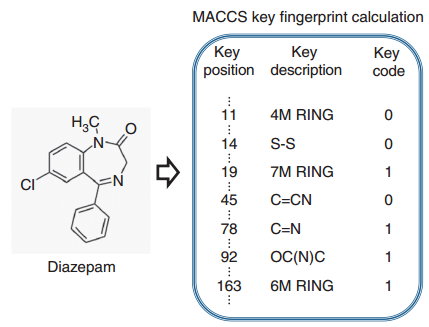
\includegraphics[scale=0.85]{section1/fing.png}
	\caption{نمایش نحوه ساخت اثر انگشت دارو}
	\label{fs6}
\end{figure} 

\end{definition}

\begin{definition}{خارج از برچسب}

برای توصیف داروی پزشکی به‌کار می‌رود. درصورتی که دارویی برای درمان بیماریی تجویز شود ولی برای درمان آن بیماری از طرف 
\LR{FDA}
تایید نشده باشد به آن نوع از استفاده، خارج از برچسب
\LTRfootnote{Off - Label}
می‌گویند. مثلا ممکن است دارویی برای معالجه کودک تایید شود اما از آن برای درمان بزرگسالان استفاده شود. نمونه‌ی دیگری از خارج از برچسب در بخش 
\ref{sideeffect}
معرفی می‌شود.
\end{definition}

\subsection{ساختار شیمیایی}

881 نوع زیرساختار مختلف تعریف شده است که یک دارو ممکن است آن‌ها را داشته یا نداشته باشد.  ساختار شیمیایی داروها در پایگاه داده‌های دارو نظیر 
\lr{DrugBank}
 یا 
\lr{PubChem}\cite{Y. Wang2009}
 در قالب فایل 
\lr{mol}،
\lr{smiles}
 و 
\lr{sdf}
 وجود دارند. در شکل
\ref{fs4} 
ساختار شیمیایی داروی دیازپام نشان‌داده شده ‌است.

\begin{figure}
	\centering
	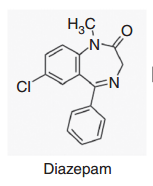
\includegraphics[scale=0.99]{section1/chem.png}
	\caption{	
	 ساختار شیمیایی داروی دیازپام }
	\label{fs4}
\end{figure}

\subsection{عوارض‌جانبی}
\label{sideeffect}

داروها می‌توانند عوارض‌جانبی ایجاد کنند. برخلاف تصور عموم، که عوارض‌جانبی دارو را فقط مختص مصرف خودسرانه‌ی دارو می‌دانند، باید دانست که عوارض‌جانبی بر اثر مصرف همه‌ی انواع داروها ایجاد می‌شوند؛ هم داروهایی که توسط پزشک تجویز شده‌اند و هم داروهایی که بدون نسخه تهیه می‌شوند. برای مثال، برخی آنتی‌بیوتیک‌ها مثل خانواده‌ی پنی‌سیلین‌ها، می‌توانند در افراد واکنش‌های حساسیتی ایجاد کنند. دانه‌های ریزپوستی
\LTRfootnote{Skin Rash}،
شایع‌ترین عارضه‌ی واکنش‌های حساسیتی به پنی‌سیلین‌ها و آنافیلاکسی مهم‌ترین یا خطرناک‌ترین عارضه‌ی ثانویه‌ی مصرف پنی‌سیلین‌ها به‌شمار می‌روند.
در این‌جا عوارض‌جانبی به دو دسته‌ی زیر تقسیم‌بندی می‌شوند:

عوارض جانبی برچسب‌دار
\LTRfootnote{Label Side Effect} 

عوارض جانبی خارج از برچسب
\LTRfootnote{Off-Label Side Effect}

\subsection{آنزیم‌}

بسیاری از داروها اثر خود را از طریق انجام واکنش با آنزیم‌ها
\LTRfootnote{Enzymes}
 اعمال می‌کنند. 
\lr{Cytochrome P450}
یک خانواده گسترده از آنزیم‌های هموپروتئینی است که در تمام موجودات زنده وجود دارد و ایزوآنزیم
\lr{CYP}
بیشتر متابولیسم داروها را انجام می‌دهد. همچنین فعال‌شدن بسیاری ترکیبات شیمیایی در درون بدن توسط همین ایزوآنزیم‌ها انجام می‌گیرد.
  
\subsection{منتقل کننده‌}

انتقال دارو یک موضوع حیاتی در پزشکی و درمان است. انتقال داروی کنترل‌شده، دسترسی به دارو را به واسطه جلوگیری از تجزیه در زمان نامناسب، افزایش دریافت دارو، حفظ غلظت دارو در طی درمان به واسطه کنترل سرعت آزادسازی دارو و کاهش عوارض جانبی از طریق هدفمندی دارو به جایگاه و سلول خاص را بهبود می‌بخشد. برای کاهش میزان تجزیه‌ی دارو، جلوگیری از عوارض جانبی مضر، افزایش دسترسی به دارو و تجمع دارو در ناحیه هدف، سیستم‌های متنوع انتقال و هدفمندی دارو در حال پیشرفت است. برای آزادسازی پیوسته‌ی دارو بایستی از پلیمرهایی استفاده کرد که دارو را با سرعتی قابل کنترل منتشر کنند یا با تجزیه‌ی پلیمر طی زمان آزاد شوند. در بین حامل‌های دارویی می‌توان پلیمرهای محلول، میکرو ذرات تشکیل شده از پلیمرهای طبیعی و سنتزی غیرمحلول و تجزیه‌پذیر، میکروکپسول‌ها، سلول‌ها، لیپوپروتئین‌ها، لیپوزوم‌ها و میسل‌ها را نام برد. حامل‌ها می‌توانند تجزیه پذیر، القایی (مثلا حساس به دما)، و حتی با تعبیه آنتی‌بادی خاص علیه ترکیبات ناحیه‌ی موردنظر هدفمند شوند.

\subsection{پروتیئن هدف}

ممکن است دارو به پروتئین‌های مختلفی بچسبد. در طراحی دارو به این نکته توجه می‌شود که از لحاظ هندسی دارو مکمل پروتئین هدف باشد تا بتواند به خوبی به آن متصل شود.

\subsection{نشانگان}

به بیماری‌هایی که دارو برای آنها تجویز می‌شود نشانگان
\LTRfootnote{Indication}
 گفته‌ می‌شود، ممکن‌ است یک دارو در درمان چند نوع بیماری موثر باشد.

\subsection{برهم‌کنش غذا - دارو}

برهم‌کنش غذا - دارو
\LTRfootnote{Food - Drug Interaction}
در اثر واکنش بین دارو و مواد خاص خوردنی یا نوشیدنی به وجود می‌آید. مثلاً آهن و کلسیم موجود در خوراکیها، مکمل‌های ویتامینی و داروهای ضد اسید معده، در معده به آنتی‌بیوتیک‌ها چسبیده و از جذب آنها به داخل خون جلوگیری می‌کنند. به‌عنوان یک مثال ساده‌، می‌توان ممنوعیت مصرف آنتی‌بیوتیک خوراکی همراه با شیر را ذکر کرد.

\subsection{ویژگی های سه بعدی }

ساختار شیمیای سه بعدی داروها
\LTRfootnote{3-D Drug Chemical Structure}
اطلاعاتی از نوع اتم‌ها و نحوه‌ی جای‌گیری آن‌ها در فضا ارائه می‌دهد. این ویژگی‌ها با استفاده از نرم‌افزار‌های خاصی اندازه‌گیری می‌شوند.



\par
\section{تعریف مسئله}
هنگامی که پزشک به‌طور همزمان چند دارو برای یک بیمار تجویز می‌کند، برهم‌کنش دارو–دارو  ممکن است عوارض‌جانبی جبران‌ناپذیری ایجاد کند، به‌طور مثال ممکن است تاثیرات داروها بر روی یکدیگر منجر به بیماری‌ها‌ی دیگر و یا حتی مرگ شود. این تاثیرات جانبی به‌طور خاص در افراد پیر و بیماران سرطانی که در روز تعداد زیادی دارو مصرف می‌کنند، چشم‌گیرتر است. عوارض‌جانبی یک دارو تا حد قابل قبولی در فاز توسعه دارو شناسایی می‌شود ولی عوارض‌جانبی حاصل از برهم‌کنش دارو–دارو  به دلیل دامنه گسترده مسئله به‌ندرت کشف می‌شود. چنین تاثیراتی عمدتا پس از تایید دارو و ورود دارو به بازار مصرف شناسایی می‌شوند که این خطری جدی برای سلامتی بیماران است. این مسئله از نظر اقتصادی نیز مهم ‌است زیرا پس از شناسایی برهم‌کنش مخرب یک دارو با داروی دیگر، ممکن‌ است آن دارو به طور کل از بازار جمع‌آوری شود. از طرفی به‌دلیل پرهزینه بودن روش‌های آزمایشگاهی، از مدل‌های پیش‌بینی برهم‌کنش دارو–دارو  استفاده می‌کنند. برای این مسئله تا‌کنون روش‌های متنوع محاسباتی، آماری، یادگیری‌ماشین و غیره ارائه شده‌است. در این پایان‌نامه روشی نوین برای حل این مسئله ارائه می‌دهیم.
 
\subsection{برچسب برهم‌کنش‌ها}  

به‌طور‌کلی به برهم‌کنش دارو–دارو  یکی از دو برچسب زیر را نسبت می‌دهند:

\textbf{برچسب مثبت}:
اگر وجود برهم‌کنش بین دو دارو با شواهد موجود ثابت شده‌ باشد و حداقل در یکی از پایگاه داده‌های دارو ثبت شده‌ باشد.

\textbf{برچسب منفی}:
برهم‌کنش دارو–داروهایی در این دسته قرار‌ می‌گیرند که تاکنون شناخته‌ نشده‌اند و در هیچ‌یک از پایگاه داده‌های مربوط به دارو ثبت نشده‌اند. در‌واقع با گذشت زمان ممکن‌ است شواهدی مبنی‌بر وجود برهم‌کنش بین دو دارو یافت شود و این برهم‌کنش برچسب مثبت بگیرد، اما تاکنون چنین اطلاعاتی در دست نیست.
\par
در این پایان‌نامه،به برهم‌کنش دارو–دارو  یکی از سه برچسب زیر را نسبت می‌دهیم:

\textbf{برچسب مثبت یک}:
اگر وجود برهم‌کنش بین دو دارو با شواهد موجود افزاینده باشد و حداقل در یکی از پایگاه داده‌های دارو ثبت شده‌ باشد.

\textbf{برچسب منفی یک}:
اگر وجود برهم‌کنش بین دو دارو با شواهد موجود کاهنده باشد و حداقل در یکی از پایگاه داده‌های دارو ثبت شده‌ باشد.

\textbf{برچسب صفر}:
اگر وجود برهم‌کنش بین دو دارو تاکنون شناخته نشده‌ باشد و در هیچ‌یک از پایگاه داده‌های دارو ثبت نشده‌ باشد.

\par 

\section{ساختار پایان‌نامه}
در ادامه‌ی این پایان‌نامه، ابتدا در فصل دو به بررسی پیشینه‌ی تحقیق و کار‌های انجام‌شده برروی داد‌ه‌های سه کلاسه از برهم کنش دارو - دارو می‌پردازیم. در مرحله‌ی بعد مفاهیم پیش نیاز برای ارائه روش پیشنهادی خود را معرفی می‌کنیم. این مفاهیم شامل دو بخش آماده‌سازی داده و رویکرد عمده‌ی انتخاب مدل می‌باشد.

در فصل سه، مجموعه‌داده‌ی به‌کار‌رفته را شرح خواهیم داد و روش پیشنهادی خود را با شرح مبسوط فرآیند کار برای حل مساله  مطرح خواهیم کرد. 

در فصل چهار به تحلیل و ارزیابی و بحث روی نتایج خواهیم پرداخت. در ادامه و در فصل پنج روش‌های پیشنهادی و کارهای آتی در جهت بهبود ارائه می‌شوند.

 
